\section{Almost generalised gamma convolutions}\label{ch:almost}

Below the basepoint one, as Section~\ref{bp:sec:compare} concluded, every positive object built so far from the shifted clock $T_\alpha$, whose Laplace transform is $\varphi_\alpha(u)=\xi(\alpha)/\xi(\alpha+\sqrt u)$, is equivalent, up to the boundary case, to the absence of zeros in the half plane $\re s>\alpha$. These equivalences are restatements rather than reductions. Since no zero free half plane was known before 2026, and none is known to the left of the line $\re s=\frac78$ (Section~\ref{sec:ch25:open}), the question that remains is quantitative: how negative can the Thorin density be below the basepoint one? Zero density estimates answer it with no hypothesis: with those of Ingham, of Guth and Maynard and of Huxley, every $T_\alpha$ with $\alpha>\frac12$ is a GGC up to a defect carried by the zeros to the right of $\alpha$, whose Cauchy kernels carry a vanishing fraction of the mass of the others, with a power saving; we call this property almost GGC.

With $\xi$ again in place of $\xi(\cdot,\chi_{12})$, we keep the notation of Sections~\ref{ch:basepoint} and \ref{ch:sato}: $v_\alpha(\theta)=\re(\xi'/\xi)(\alpha+i\theta)$, and the Thorin density at the basepoint $\alpha$ in the chart $\theta=\sqrt z$ is $v_\alpha/\pi$, the density $\rho_{\alpha-1/2}$ of \eqref{eq:rho} at the resolution $\alpha-\frac12$; in this section the basepoint, not the resolution, is the index. $P_w(x)=w/(\pi(w^2+x^2))$ is the Poisson kernel of Section~\ref{ch:clock}, $P_{-w}=-P_w$, and $P_0$ is the unit point mass, as in Proposition~\ref{prop:signature}. A zero is $\rho=\beta+i\gamma$; $N(T)$ counts the zeros with $0<\gamma\le T$, and $N(\sigma,T)$ those among them with $\beta\ge\sigma$, so that $N(\sigma,T)\ge\nu(\sigma,T)$ in the notation of Proposition~\ref{prop:zerodensity}.

\subsection{Mass bookkeeping and the almost GGC theorem}\label{ag:sec:almost}

The Poisson form of Proposition~\ref{prop:struct} splits according to the side of the line $\re s=\alpha$ on which each zero lies, $v_\alpha=v_\alpha^+-v_\alpha^-$, with
\begin{equation}\label{ag:eq:split}
\begin{aligned}
\frac{v_\alpha^+(\theta)}\pi&=\sum_{\beta\le\alpha,\ \gamma>0}\big[P_{\alpha-\beta}(\theta-\gamma)+P_{\alpha-\beta}(\theta+\gamma)\big],\\
\frac{v_\alpha^-(\theta)}\pi&=\sum_{\beta>\alpha,\ \gamma>0}\big[P_{\beta-\alpha}(\theta-\gamma)+P_{\beta-\alpha}(\theta+\gamma)\big].
\end{aligned}
\end{equation}
Both parts are positive, and a zero on the line $\re s=\alpha$, if there is one, contributes a unit atom at its ordinate to the positive part. Each pair of kernels has mass one on $(0,\infty)$. A zero with $\beta>\alpha$ has the partner $1-\bar\rho=1-\beta+i\gamma$, whose real part $1-\beta<\frac12<\alpha$ puts it in the positive part. Write $m_\alpha^\pm(T)=\pi^{-1}\int_0^Tv_\alpha^\pm(\theta)\,d\theta$ for the positive and negative masses on $[0,T]$.

\begin{lemma}[Mass bookkeeping]\label{ag:lem:mass}
Let $\alpha>\frac12$, and suppose that $N(\alpha,t)\le t^{e+o(1)}$ as $t\to\infty$ for some $e<1$. Then
\[
m_\alpha^-(T)\le N(\alpha,2T)+O\big(T^{e-1+o(1)}\big),\qquad m_\alpha^+(T)=\frac T{2\pi}\log\frac T{2\pi}+O(T).
\]
\end{lemma}

\begin{proof}
A zero with $\beta>\alpha$ and $\gamma\le2T$ contributes at most its total mass one. For a zero with $\gamma>2T$ put $w=\beta-\alpha$, so that $0<w<\frac12$. Since $\int_0^TP_w(\theta+\gamma)\,d\theta=\int_{-T}^0P_w(\theta-\gamma)\,d\theta$, its pair of kernels has mass on $[0,T]$ at most
\[
\int_{-\infty}^TP_w(\theta-\gamma)\,d\theta\le\frac{w}{\pi(\gamma-T)}\le\frac1{\pi\gamma},
\]
and $\sum_{\beta>\alpha,\ \gamma>2T}\gamma^{-1}=\int_{2T}^\infty t^{-1}dN(\alpha,t)\le\int_{2T}^\infty N(\alpha,t)t^{-2}dt\ll T^{e-1+o(1)}$. The positive part contains the kernels of all zeros with $\beta\le\alpha$, among them every zero on the critical line and every partner $1-\bar\rho$. Its mass on $[0,T]$ is therefore $N(T)$ up to the $N(\alpha,T)=O(T^{e+o(1)})$ zeros to the right of $\alpha$, whose kernels it lacks, and up to the tails of the kernels of the zeros near height $T$, which change it by $O(\log^2T)$. Since $N(T)=\frac T{2\pi}\log\frac T{2\pi}-\frac T{2\pi}+O(\log T)$, the second claim follows.
\end{proof}

\begin{theorem}[Almost GGC]\label{ag:thm:almost}
For every $\frac12<\alpha<1$, with no hypothesis,
\[
\frac{m_\alpha^-(T)}{m_\alpha^+(T)}\le T^{e(\alpha)-1+o(1)},\qquad e(\alpha)=\begin{cases}\dfrac{3(1-\alpha)}{2-\alpha},&\frac12<\alpha<\frac7{10},\\[2ex]\dfrac{15(1-\alpha)}{3+5\alpha},&\frac7{10}\le\alpha<1,\end{cases}
\]
and $e(\alpha)<1$ throughout, so the negative part $v_\alpha^-/\pi$ of \eqref{ag:eq:split}, the Cauchy kernels of the zeros to the right of $\alpha$, carries on $[0,T]$ a vanishing fraction of the mass of the positive part, with a power saving. For $\alpha\ge1$ no zero lies to the right of $\alpha$, and $m_\alpha^-=0$. Under the density hypothesis $e(\alpha)=2(1-\alpha)$. RH holds if and only if $v_\alpha^-$ vanishes identically for every $\alpha>\frac12$.
\end{theorem}

\begin{proof}
Combine Lemma~\ref{ag:lem:mass} with three zero density estimates: Ingham's $N(\sigma,T)\ll T^{3(1-\sigma)/(2-\sigma)}\log^5T$ \cite{Ingham40}; Guth and Maynard's $N(\sigma,T)\le T^{15(1-\sigma)/(3+5\sigma)+o(1)}$ for $\frac7{10}\le\sigma\le\frac45$ \cite[Theorem 1.2]{GM26}; and Huxley's $N(\sigma,T)\le T^{3(1-\sigma)/(3\sigma-1)+o(1)}$ for $\sigma\ge\frac34$ \cite{Huxley72}, whose exponent is at most $15(1-\sigma)/(3+5\sigma)$ when $\sigma\ge\frac45$. Since $3(1-\alpha)<2-\alpha$ exactly when $\alpha>\frac12$, and $15(1-\alpha)<3+5\alpha$ exactly when $\alpha>\frac35$, the exponent is below one for every $\frac12<\alpha<1$. Finally, $v_\alpha^-$ vanishes identically exactly when no zero has $\beta>\alpha$, which is the GGC criterion of Theorem~\ref{thm:poisson}.
\end{proof}

Even the classical estimate of Bohr and Landau \cite{BL14}, $N(\sigma,T)=O(T)$ for fixed $\sigma>\frac12$, gives a vanishing fraction $O(1/\log T)$; the zero density estimates improve this to a power of $T$. First, the theorem bounds the decomposition mass $m_\alpha^-(T)$, which overcounts the negative part $\int_0^T\max(-v_\alpha/\pi,0)\,d\theta$ of the density itself, because the positive kernels of nearby zeros cancel much of each negative kernel. The partner of a zero already cancels part of it: with $\varepsilon=\alpha-\frac12$ and $\delta=\beta-\frac12$, twice the mass in Proposition~\ref{prop:signature}(iii) gives the negative part of $P_{\alpha+\beta-1}-P_{\beta-\alpha}=P_{\varepsilon+\delta}+P_{\varepsilon-\delta}$ the mass $\frac4\pi\arctan\sqrt{(\delta+\varepsilon)/(\delta-\varepsilon)}-1=\frac2\pi\arcsin\frac\varepsilon\delta$, less than the mass one that the decomposition counts, and Section~\ref{ag:sec:num} shows the effect of the other zeros. Second, on the verified range the negative mass is essentially zero. All zeros with $0<\gamma\le T_0$ lie on the critical line \cite{PT21}, so for $T\le T_0/2$ the only negative contributions come from zeros above $T_0$, and by the proof of Lemma~\ref{ag:lem:mass} their total mass on $[0,T]$ is $O(T_0^{e(\alpha)-1+o(1)})$.

The left panel of Figure~\ref{ag:fig:almost} draws the exponents. The saving $1-e(\alpha)$ is small near the centre, where Ingham's exponent gives $(2\alpha-1)/(2-\alpha)$. Sharper exponents are known near $\alpha=1$: the density hypothesis itself holds for $\alpha>\frac{25}{32}$ \cite[p.~133]{Bourgain00}, and Huxley's exponent \cite{Huxley72} is $0.176$ at $\alpha=0.9$; those of the theorem suffice for what follows.

\subsection{The canonical factorisation and explicit unconditional bounds}\label{ag:sec:factor}



\begin{proposition}[Canonical factorisation]\label{ag:prop:factor}
For every $\alpha>\frac12$ and $u\ge0$, $\varphi_\alpha(u)=\varphi_\alpha^+(u)\,D_\alpha(u)$, where
\begin{gather*}
\varphi_\alpha^+(u)=\exp\Big\{-\int_0^\infty\log\Big(1+\frac u{\theta^2}\Big)\frac{v_\alpha^+(\theta)}\pi\,d\theta\Big\},\\
D_\alpha(u)=\prod_{\beta>\alpha,\ \gamma>0}\frac{(\beta-\alpha)^2+\gamma^2}{(\sqrt u-\beta+\alpha)^2+\gamma^2};
\end{gather*}
here $\varphi_\alpha^+$ is the Laplace transform of a GGC $T_\alpha^+$ with Thorin density $v_\alpha^+/\pi$ in the chart $\theta=\sqrt z$, and the product defining the defect $D_\alpha$ runs over the zeros to the right of the line $\re s=\alpha$ and converges absolutely. The defect is identically one if and only if $\zeta$ has no zeros with $\re s>\alpha$, and then $T_\alpha\stackrel d=T_\alpha^+$. Otherwise $D_\alpha(u)\to0$ as $u\to\infty$, and $T_\alpha^+$ is not the sum of $T_\alpha$ and an independent nonnegative variable.
\end{proposition}

\begin{proof}
Grouping the Hadamard product of $\xi$ in conjugate pairs, as in the proof of Proposition~\ref{prop:struct}, gives for $u\ge0$
\[
\varphi_\alpha(u)=\prod_{\gamma>0}\frac{(\alpha-\beta)^2+\gamma^2}{(\alpha-\beta+\sqrt u)^2+\gamma^2},
\]
over the zeros with $\gamma>0$, counted with multiplicity; each factor is $1+O((u+\sqrt u)\gamma^{-2})$ and $\sum\gamma^{-2}<\infty$, so the product converges absolutely. For $\beta<\alpha$, with $w=\alpha-\beta>0$, the factor is $(w^2+\gamma^2)/((w+\sqrt u)^2+\gamma^2)=\exp\{-\int_0^\infty\log(1+u/\theta^2)[P_w(\theta-\gamma)+P_w(\theta+\gamma)]\,d\theta\}$, the Laplace transform of a GGC whose Thorin density is the pair of Cauchy kernels of width $w$ at $\pm\gamma$ (the computation after Theorem~\ref{sm:thm:thorin}); for $\beta=\alpha$ it is $\gamma^2/(\gamma^2+u)$, an exponential law, whose Thorin measure is the atom at $\gamma$. The partial products over the zeros with $\beta\le\alpha$ are therefore Laplace transforms of GGCs, they converge for every $u\ge0$ to a limit continuous at the origin, and by the closure theorem of Section~\ref{sec:weak:limits} the limit is the Laplace transform of a GGC, with Thorin density $v_\alpha^+/\pi$. The remaining factors form $D_\alpha$. If a zero lies to the right of $\alpha$, put $w=\beta-\alpha\in(0,\frac12)$; its factor tends to zero as $u\to\infty$, and every factor of $D_\alpha$ is at most one for $u\ge1$, because $(\sqrt u-w)^2\ge w^2$ when $\sqrt u\ge2w$. So $D_\alpha(u)\to0$. If $T_\alpha^+$ were $T_\alpha+S$ with $S\ge0$ independent of $T_\alpha$, then $\E e^{-uS}=\varphi_\alpha^+(u)/\varphi_\alpha(u)=1/D_\alpha(u)$ would be unbounded, which is impossible.
\end{proof}

The proposition also says what the signed density $v_\alpha/\pi$ is. When every zero lies to the left of the line $\re s=\alpha$ it is the Thorin density of $T_\alpha$ (Theorem~\ref{thm:poisson}); a zero on the line adds to the Thorin measure an atom at its ordinate, the term $P_0$ of \eqref{ag:eq:split}, which the function $v_\alpha$ does not show. When a zero lies to the right of the line, $T_\alpha$ is not a GGC and $v_\alpha/\pi$ is not a signed Thorin density for it in any sense: the negative kernel $-P_w$ of such a zero integrates to the factor $((w+\sqrt u)^2+\gamma^2)/(w^2+\gamma^2)$, while the zero contributes $(w^2+\gamma^2)/((\sqrt u-w)^2+\gamma^2)$ to $\varphi_\alpha$. The bookkeeping of Theorem~\ref{ag:thm:almost} applies to the other reformulations in Chapters~\ref{chap:basepoint} to \ref{chap:almost}. In the normal scale mixture of Theorem~\ref{sm:thm:strip} it bounds the negative part of the candidate EGGC density $v_\alpha/\pi$; in Wiener's theorem (Proposition~\ref{wr:prop:wiener}) it bounds the proportion of frequencies at which the Fourier transform of the tilted P\'olya kernel can vanish; and in Riesz's criterion (Section~\ref{wr:sec:riesz}) it bounds the number of Mellin poles to the right of $\alpha/2$.

The pole factors can be written down. Let $U_\alpha^\circ$ denote the signed measure on $\theta>0$ with density $v_\alpha/\pi$ and a unit atom at $\gamma$ for every zero $\beta+i\gamma$, $\gamma>0$, with $\beta=\alpha$ (the term $P_0$ of \eqref{ag:eq:split}), counted with multiplicity.

\begin{theorem}[Signed Thorin representation]\label{tx:thm:signed}
For every $\alpha\ge\frac12$ and $u\ge0$,
\[
\varphi_\alpha(u)=\exp\Big\{-\int_0^\infty\log\Big(1+\frac u{\theta^2}\Big)U_\alpha^\circ(d\theta)\Big\}\prod_{\beta>\alpha,\ \gamma>0}\Big|1-\frac u{(\rho-\alpha)^2}\Big|^{-2},
\]
the integral and the product converging absolutely. For a zero to the right of $\alpha$, with $p=(\rho-\alpha)^2=-c+id$, $c=\gamma^2-(\beta-\alpha)^2>0$ and $d=2\gamma(\beta-\alpha)>0$, the factor is
\[
\Big|1-\frac up\Big|^{-2}=\frac{|p|^2}{(u+c)^2+d^2}=|p|^2\int_0^\infty e^{-ut}\,\frac{e^{-ct}\sin dt}d\,dt,
\]
the Laplace transform of a damped sinusoid, which changes sign, so the factor is not completely monotone.
\end{theorem}

\begin{proof}
Write $f_w(u)=(w^2+\gamma^2)/((w+\sqrt u)^2+\gamma^2)$. By the Hadamard product, as in the proof of Proposition~\ref{ag:prop:factor}, $\varphi_\alpha(u)=\prod_{\gamma>0}f_{\alpha-\beta}(u)$ over all zeros with $\gamma>0$, absolutely convergent. For $w\ge0$ that proof gives $f_w(u)=\exp\{-\int_0^\infty\log(1+u/\theta^2)[P_w(\theta-\gamma)+P_w(\theta+\gamma)]\,d\theta\}$, with the atom at $\gamma$ for $w=0$. For $w=-\omega<0$ the kernels carry the sign $P_{-\omega}=-P_\omega$, so the same integral equals $f_\omega^{-1}$, and a direct computation gives $f_{-\omega}=f_\omega^{-1}\,|p|^2/|p-u|^2$ with $p=(\omega+i\gamma)^2$, since $|p-u|^2=((\sqrt u-\omega)^2+\gamma^2)((\sqrt u+\omega)^2+\gamma^2)$. Multiplying over the zeros gives the formula, once the integrals are summed under the integral sign: the integral of each pair of kernels against $\log(1+u/\theta^2)$ is $\pm\log f_{|w|}$, which is $O_\alpha((u+\sqrt u)\gamma^{-2})$, and $\sum\gamma^{-2}<\infty$. Finally $|p-u|^2=(u+c)^2+d^2$, and $c>0$ because $\beta-\alpha<\frac12<\gamma_1$.
\end{proof}

The theorem needs no hypothesis on the zeros: the atoms carry the zeros on the line $\re s=\alpha$, which is why the case $\alpha=\frac12$ is included. It is the identity behind Proposition~\ref{ag:prop:factor}, which combines the pole factors with the negative kernels they cancel into $D_\alpha$. At $\alpha=\frac12$ every term is explicit.

\begin{corollary}[The critical line]\label{tx:cor:half}
Unconditionally, $U_{1/2}^\circ=\sum_{\beta=1/2,\ \gamma>0}\delta_\gamma\ge0$ and
\[
\varphi_{1/2}(u)=\prod_{\beta=1/2,\ \gamma>0}\frac{\gamma^2}{\gamma^2+u}\ \prod_{\beta>1/2,\ \gamma>0}\Big|1-\frac u{(\rho-\frac12)^2}\Big|^{-2}.
\]
\end{corollary}

\begin{proof}
A zero $\rho$ with $\beta=\frac12+\delta$, $\delta>0$, and its partner $1-\bar\rho$ have the same ordinate, and their kernels $P_{-\delta}+P_\delta$ cancel, so $v_{1/2}=0$ away from the atoms (the term by term form in the proof of Proposition~\ref{prop:struct}, which holds at $\alpha=\frac12$ away from the ordinates). The atoms come from the zeros with $\beta=\frac12$, each with the factor $f_0=\gamma^2/(\gamma^2+u)$; apply Theorem~\ref{tx:thm:signed}.
\end{proof}

So on the critical line positivity of $U_{1/2}^\circ$ costs nothing, and RH is the statement that the product of damped sinusoids is empty. For $\frac12<\alpha<\sup_\rho\re\rho$ the negative kernels of Proposition~\ref{ag:prop:factor} are present, and whether they can be outweighed on the single line $\re s=\alpha$ is open, except near a zero, where they cannot (Remark~\ref{rem:ch2:oneline}).

\begin{theorem}[Explicit bounds from verification]\label{ag:thm:explicit}
Let $T_0=3\times10^{12}$, below which all zeros lie on the critical line \cite{PT21}, and let $\Sigma_0=\sum_{\gamma>T_0}\gamma^{-2}$, the sum over all zeros above $T_0$, counted with multiplicity. By the Riemann von Mangoldt formula with the explicit error term of Hasanalizade, Shen and Wong \cite{HSW22}, recalled in the proof of Proposition~\ref{bp:prop:v1min}, $\Sigma_0$ differs from $\frac{\log(T_0/2\pi)+1}{2\pi T_0}=1.4797\times10^{-12}$ by less than $2\times10^{-24}$, so $\Sigma_0<1.48\times10^{-12}$. Then for every $\alpha>\frac12$ and every $u\ge0$:
\begin{enumerate}
\item $|\log D_\alpha(u)|\le(u+\sqrt u)\,\Sigma_0$, so that
\[
e^{-1.5\times10^{-12}(u+\sqrt u)}\,\varphi_\alpha^+(u)\le\E e^{-uT_\alpha}\le e^{1.5\times10^{-12}(u+\sqrt u)}\,\varphi_\alpha^+(u);
\]
\item the negative part of the density satisfies $v_\alpha^-(\theta)/\pi\le2\Sigma_0/\pi<9.43\times10^{-13}$ for $0\le\theta\le T_0/2$;
\item consequently $v_\alpha(\theta)>0$ for all $0\le\theta\le T_0/2$ whenever $\alpha-\frac12>6\times10^{-10}$.
\end{enumerate}
\end{theorem}

\begin{proof}
Every zero to the right of $\alpha$ has $\gamma>T_0$ and $\beta>\frac12$. The zeros above $T_0$ off the critical line come in pairs $\beta+i\gamma$, $1-\beta+i\gamma$ of equal multiplicity, by $\xi(s)=\xi(1-s)$ and $\xi(\bar s)=\overline{\xi(s)}$, and at most one member of each pair lies to the right of $\alpha$, so $\sum_{\beta>\alpha,\ \gamma>0}\gamma^{-2}\le\Sigma_0/2$. (1) For a zero to the right of $\alpha$ put $w=\beta-\alpha\in(0,\frac12)$ and $x=(u-2w\sqrt u)/(w^2+\gamma^2)$, so that its factor in $D_\alpha$ is $1/(1+x)$. Since $u-2w\sqrt u\ge-w^2$, we have $x\ge-w^2/\gamma^2>-\frac12$, and $|x|\le(u+\sqrt u)/\gamma^2$; for $x\ge-\frac12$, $|\log(1+x)|\le2|x|$. Hence the logarithm of its factor is at most $2(u+\sqrt u)/\gamma^2$ in absolute value, and summing gives $|\log D_\alpha(u)|\le(u+\sqrt u)\Sigma_0$; the inequalities for $\E e^{-uT_\alpha}=\varphi_\alpha^+(u)D_\alpha(u)$ follow. (2) For $\theta\le T_0/2$ and $\gamma>T_0$, $P_w(\theta-\gamma)+P_w(\theta+\gamma)\le\frac{2w}{\pi(\gamma-\theta)^2}\le\frac4{\pi\gamma^2}$, and summing over the zeros to the right of $\alpha$ gives at most $\frac4\pi\cdot\frac{\Sigma_0}2$. (3) Write $a=\alpha-\frac12$. If $a\ge\frac12$, then $\alpha\ge1$, no zero lies to the right of $\alpha$, and $v_\alpha=v_\alpha^+>0$; so let $6\times10^{-10}<a<\frac12$. The zeros below $T_0$ lie on the line and contribute to $v_\alpha^+/\pi$ the kernels $P_a(\theta-\gamma)$, and all other kernels of $v_\alpha^+$ are positive, so $v_\alpha^+(\theta)/\pi\ge\frac a{\pi(a^2+\gamma_1^2)}$ at every $\theta$ within $\gamma_1$ of an ordinate below $T_0$. Every $\theta\in[0,T_0/2]$ is such a point. On $[0,\gamma_1]$ the ordinate $\gamma_1$ serves. On $[\gamma_1,2000]$ one of the first $1800$ ordinates serves: they are the certified zeros of the proof of Proposition~\ref{bp:prop:v1min}, they reach height $2304.3$, and consecutive ones differ by less than $6.8874<2\gamma_1$. For $2000\le\theta\le T_0/2$, the count of that proof, with $H=14$ in place of $15$, shows that the window $(\theta-14,\theta+14]$ holds at least $n(\theta)=\frac{14}\pi\log\frac{\theta-14}{2\pi}-E(\theta-14)-E(\theta+14)$ zeros; while $\theta+14\le X_0$, $n$ increases and $n(2000)>20$, and for $\theta+14>X_0$, $n(\theta)>\frac{14}\pi\log\frac{\theta-14}{2\pi}-0.6\log(\theta+14)>80$, so the window holds a zero, which lies within $14<\gamma_1$ of $\theta$ and, since $\theta+14<T_0$, on the line. The script \texttt{explicit\_bounds.py}, with output \texttt{explicit\_bounds.json}, recomputes the $1800$ zeros and checks these inequalities in ball arithmetic. Finally, since $a<\frac12$,
\[
\frac a{\pi(a^2+\gamma_1^2)}>\frac a{\pi(\frac14+\gamma_1^2)}>\frac{6\times10^{-10}}{\pi(\frac14+\gamma_1^2)}>9.5\times10^{-13},
\]
which is more than the bound $2\Sigma_0/\pi<9.43\times10^{-13}$ of (2) on $v_\alpha^-/\pi$, so $v_\alpha=v_\alpha^+-v_\alpha^->0$ on $[0,T_0/2]$.
\end{proof}

Theorem~\ref{ag:thm:explicit} restates the verification of RH to height $3\times10^{12}$ in Thorin form. Part (3) of Theorem~\ref{sm:thm:strip} is the same statement for the characteristic function of the normal scale mixture, with a remainder of relative size $\log T_0/T_0$, and the paragraph after its proof bounds the negative part of $v_\alpha/\pi$ for $\theta\le10^9$ in the same way as part (2).

Part (3) of Theorem~\ref{ag:thm:explicit} treats every zero above $T_0$ as if its kernel could be negative wherever the density is evaluated. As the first author's note on the Dirichlet beta function observes \cite{P26beta}, grouping each such zero with its reflection in the critical line does better, because the sum of the two kernels of an off line pair is negative only near its ordinate.

\begin{corollary}[Positivity on the verified window]\label{cor:dbeta:window}
Let $T_0=3\times10^{12}$ and $V_\xi=(\log\xi)''(\frac12)=0.04620998623$.
\begin{enumerate}
\item For every $\alpha>\frac12$, $v_\alpha(\theta)>0$ for $|\theta|\le T_0-\frac12$.
\item For every $\alpha\in(\frac12,7.35]$, $v_\alpha(\theta)>v_\alpha(0)$ for $0<|\theta|\le T_0-\frac{1+\sqrt2}2$, and $0<v_\alpha(0)\le(\alpha-\frac12)V_\xi$.
\end{enumerate}
\end{corollary}

\begin{proof}
(1) Put $\varepsilon=\alpha-\frac12$. By the Hadamard product, as in Proposition~\ref{prop:struct}, $v_\alpha(\theta)$ is the absolutely convergent sum over the zeros $\rho=\beta+i\gamma$, counted with multiplicity, of $(\alpha-\beta)/((\alpha-\beta)^2+(\theta-\gamma)^2)$. A zero on the critical line contributes $\pi P_\varepsilon(\theta-\gamma)>0$. The zeros off the line come in pairs $\frac12\pm\delta+i\gamma$ with $0<\delta<\frac12$ and equal multiplicities, and a pair contributes $\pi(P_{\varepsilon+\delta}+P_{\varepsilon-\delta})(\theta-\gamma)$, which is nonnegative if $\delta\le\varepsilon$ and, if $\delta>\varepsilon$, negative exactly where $|\theta-\gamma|<\sqrt{\delta^2-\varepsilon^2}$, by the proof of Proposition~\ref{prop:signature}(ii); and $\sqrt{\delta^2-\varepsilon^2}<\delta<\frac12$. Every zero off the line has $|\gamma|>T_0$ \cite{PT21}, so for $|\theta|\le T_0-\frac12$ every pair has $|\theta-\gamma|>\frac12$ and contributes a nonnegative term, while the zero $\frac12+i\gamma_1$ contributes a positive one.

(2) This is Theorem~\ref{thm:dbeta:minall}(i) and (ii) for $\xi$, with $\alpha_{\max}=7.35$ and $H_0=T_0$ (Table~\ref{tab:dbeta:minall}).
\end{proof}

\begin{remark}\label{rem:dbeta:window}
The corollary does not touch the defect of part (1) of Theorem~\ref{ag:thm:explicit}: a zero above $T_0$ to the right of the line $\re s=\alpha$ stops $T_\alpha$ from being a GGC whatever $v_\alpha$ does on the window (Proposition~\ref{ag:prop:factor}), and near its own ordinate it can make $v_\alpha$ negative (Section~\ref{ag:sec:cancel}).
\end{remark}

The proof of part (1) gives, with no hypothesis, $|\log D_\alpha(u)|\le2(u+\sqrt u)\sum_{\beta>\alpha,\ \gamma>0}\gamma^{-2}$. With the verification height and the trivial count the sum is at most $\Sigma_0/2$, with $\Sigma_0<1.48\times10^{-12}$. The zero density estimates of Section~\ref{ag:sec:almost} \cite{Ingham40,GM26,Huxley72} improve this to $\sum_{\beta>\alpha}\gamma^{-2}\le\int_{T_0}^\infty t^{-2}dN(\alpha,t)\ll T_0^{e(\alpha)-2+o(1)}$, smaller by a further power of $T_0$ since $e(\alpha)<1$.

\subsection{Where negativity can come from: a cancellation lemma}\label{ag:sec:cancel}

The counting bound treats every zero to the right of $\alpha$ as if its kernel were entirely negative. Pointwise, a negative kernel is cancelled wherever the rest of the density exceeds it, and the kernel of width $w$ has height at most $1/(\pi w)$.

\begin{lemma}[Cancellation]\label{ag:lem:cancel}
Let $\rho=\beta+i\gamma$ be a zero with $\beta>\alpha$, and let $m>0$ be a lower bound on an interval $I$ for the rest of the density, $v_\alpha/\pi+P_{\beta-\alpha}(\cdot-\gamma)$. If $\beta-\alpha\ge1/(\pi m)$, the kernel of $\rho$ cannot make $v_\alpha$ negative on $I$.
\end{lemma}

\begin{proof}
On $I$, $v_\alpha/\pi\ge m-\max_xP_{\beta-\alpha}(x)=m-1/(\pi(\beta-\alpha))\ge0$.
\end{proof}

The lemma has a heuristic consequence. At height $\gamma$ the density $v_\alpha/\pi$ averages $\frac1{2\pi}\log\frac\gamma{2\pi}$, the density of the ordinates, and when $\alpha-\frac12$ is large compared with the mean spacing $2\pi/\log\gamma$ it stays close to that average. Taking this average for $m$ in the lemma, a zero to the right of $\alpha$ can then produce negativity only if
\[
\beta-\alpha<\frac{2\pi}{\pi\log(\gamma/2\pi)}=\frac2{\log(\gamma/2\pi)} .
\]
Heuristically, then, positivity of the Thorin density at the basepoint $\alpha$ can be broken at height $\gamma$ only by zeros in the thin strip $\alpha<\beta<\alpha+2/\log(\gamma/2\pi)$. The local visibility condition of Section~\ref{sec:ch13:visibility}, which concerns small resolutions, has the same scale $1/\log\gamma$. The heuristic proves nothing, because a rigorous lower bound for the background near an arbitrary height would itself control $\zeta'/\zeta$ in the strip. It suggests combining zero density estimates for thin strips with lower bounds for $\re\xi'/\xi$ on average.

We tested the lemma at the heights $300$ and $10^5$ with \texttt{high.py}. The script computes the background $v_{0.6}/\pi$ from $\xi'/\xi$ on a window of width $8$ and adds the kernels of a single hypothetical pair of zeros at $\beta+i\gamma_0$ and $1-\beta+i\gamma_0$, with $\gamma_0$ the centre of the window (Figure~\ref{ag:fig:cancel}, middle and right). At height $300$ the background has mean $0.51$ and minimum $0.069$; at height $10^5$ it has mean $1.59$, close to the density of ordinates $\frac1{2\pi}\log\frac{10^5}{2\pi}=1.54$, and minimum $0.34$. Table~\ref{ag:tab:cancel} shows the result. At both heights zeros with $\beta-\alpha\le0.2$ produce negativity and zeros with $\beta-\alpha\ge0.3$ are absorbed. At height $10^5$ the heuristic threshold $2/\log(10^5/2\pi)=0.21$ is close to the observed one, while the rigorous guarantee of Lemma~\ref{ag:lem:cancel} with the window minimum, $1/(\pi m)=0.93$, is conservative. For a fixed width the negative dip is deeper at the greater height, because the kernel is the same while the local minimum of the background near the hypothetical zero differs.

\begin{table}[htbp]
\centering\small
\begin{tabular}{ccccc}
\toprule
 & \multicolumn{2}{c}{height 300} & \multicolumn{2}{c}{height $10^5$}\\
$\beta$ & min of $v_{0.6}/\pi$ & negative mass & min of $v_{0.6}/\pi$ & negative mass\\
\midrule
0.62 & $-13.54$ & 0.521 & $-13.97$ & 0.567\\
0.65 & $-4.16$ & 0.299 & $-4.59$ & 0.365\\
0.70 & $-1.24$ & 0.121 & $-1.62$ & 0.193\\
0.75 & $-0.41$ & 0.041 & $-0.72$ & 0.097\\
0.80 & $-0.10$ & 0.008 & $-0.32$ & 0.041\\
0.90 & $0.072$ & 0 & $0.023$ & 0\\
0.95 & $0.075$ & 0 & $0.100$ & 0\\
\bottomrule
\end{tabular}
\caption{A single hypothetical pair of zeros at real parts $\beta$ and $1-\beta$ inserted into the density $v_{0.6}/\pi$, computed from $\xi'/\xi$ on a window of width $8$ at the heights $300$ and $10^5$: the minimum of the density and the negative mass $\int\max(-v_{0.6}/\pi,0)$ on the window. Computed by \texttt{high.py}.}
\label{ag:tab:cancel}
\end{table}

\subsection{Hypothetical off line zeros in the computed density}\label{ag:sec:num}

No off line zero is known, so the negative part cannot be observed. To see the mechanism, \texttt{almost.py} inserts fifteen hypothetical quadruples of zeros $0.75\pm i\gamma_j$, $0.25\pm i\gamma_j$, at the heights $\gamma_j=20\,j^{5/3}$ below $2000$, into the Poisson form of Proposition~\ref{prop:struct} together with the first $1700$ ordinates, taken on the line; the zeros above height $2198$ are omitted. The count of the hypothetical zeros grows like $T^{0.6}$, as a zero density estimate with $e=0.6$ would allow. Table~\ref{ag:tab:syn} compares the negative mass $\int_0^T\max(-v_\alpha/\pi,0)\,d\theta$ of the resulting density with its positive mass and with the counting bound $N_{\rm off}(2T)$ of Lemma~\ref{ag:lem:mass}, the number of hypothetical zeros with ordinate at most $2T$.

\begin{table}[htbp]
\centering\small
\begin{tabular}{cccccc}
\toprule
$\alpha$ & $T$ & negative mass & positive mass & fraction & counting bound $N_{\rm off}(2T)$\\
\midrule
0.6 & 250 & 0.842 & 108.8 & $7.7\times10^{-3}$ & 6\\
0.6 & 1000 & 1.655 & 650.5 & $2.5\times10^{-3}$ & 15\\
0.6 & 2000 & 2.278 & 1519.2 & $1.5\times10^{-3}$ & 15\\
0.7 & 250 & 2.130 & 110.1 & $1.9\times10^{-2}$ & 6\\
0.7 & 1000 & 4.815 & 653.6 & $7.4\times10^{-3}$ & 15\\
0.7 & 2000 & 6.938 & 1523.8 & $4.6\times10^{-3}$ & 15\\
0.8 & any & 0 & & 0 & 0\\
\bottomrule
\end{tabular}
\caption{Negative and positive mass of the density $v_\alpha/\pi$ on $[0,T]$ with fifteen hypothetical quadruples of zeros at real part $0.75$. Computed by \texttt{almost.py}.}
\label{ag:tab:syn}
\end{table}

Three features are visible. The negative mass is well below the counting bound, because each negative kernel is partly cancelled by its partner and by the positive kernels of the neighbouring zeros on the line: at $\alpha=0.6$ the negative kernel has width $0.15$ and height $1/(0.15\pi)=2.1$, and most of it is cancelled, while at $\alpha=0.7$ the width is $0.05$ and the kernel, of height $6.4$, appears as a sharp negative spike that takes the density to $-5.39$ at the height $292.40$ (Figure~\ref{ag:fig:almost}; the minimum is computed by \texttt{almost\_dip.py}). The fraction decreases with $T$ at the rate the counting predicts. And at $\alpha=0.8$, to the right of the hypothetical zeros, the density is positive everywhere, as Theorem~\ref{thm:poisson} requires: a zero with real part $\beta$ contributes a positive kernel at every basepoint $\alpha>\beta$.

A zero is most visible from basepoints just to its left. The left panel of Figure~\ref{ag:fig:cancel}, computed by \texttt{more2.py}, shows the negative mass on $[0,2000]$ as a function of $\alpha$ for the same fifteen heights and three real parts $\beta=0.6$, $0.75$ and $0.9$. As $\alpha$ increases towards $\beta$ the negative kernels narrow, cancellation fails, and the negative mass climbs towards the number of hypothetical zeros, reaching $7.55$ at $\alpha=0.85$ for $\beta=0.9$. At $\alpha=\beta$ the zeros lie on the line of evaluation and the negative mass drops to zero. This is the Thorin counterpart of the fact that the translates of the tilted P\'olya kernel fail to be complete exactly on the line through the zero (Proposition~\ref{wr:prop:wiener}).

\begin{figure}[htbp]
\centering
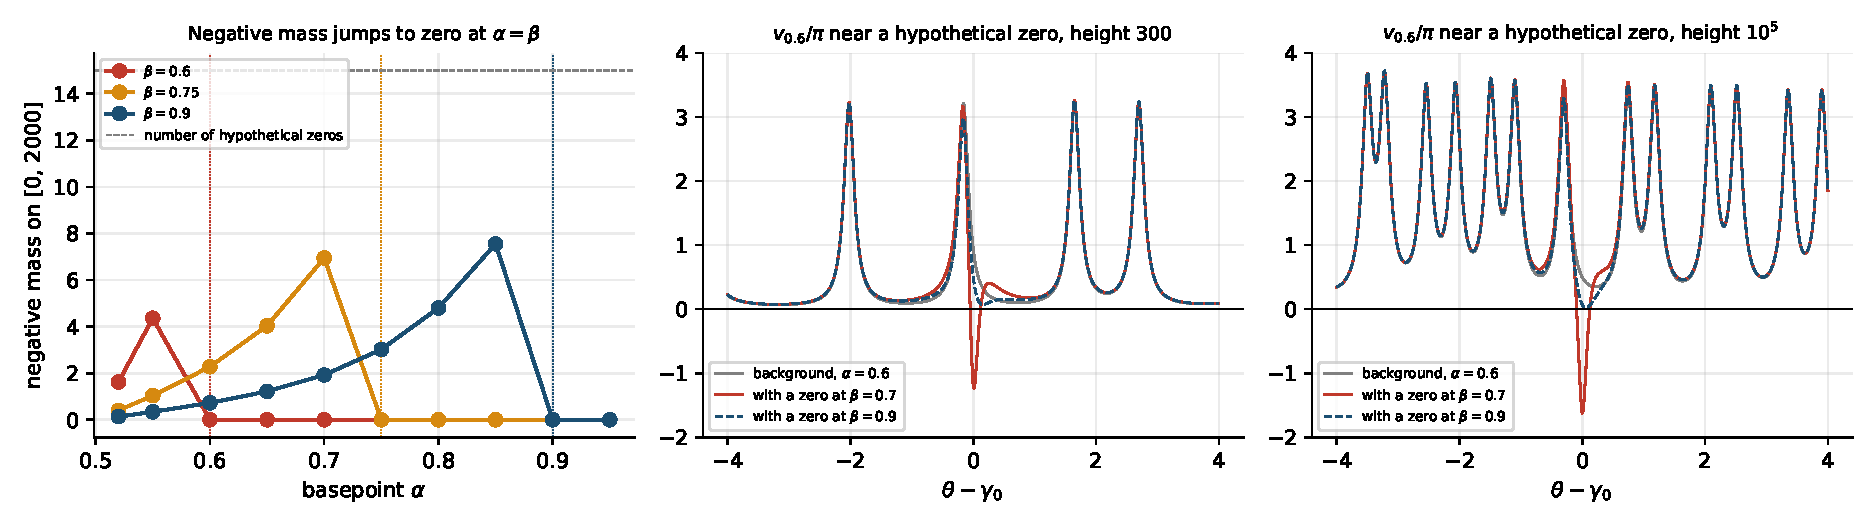
\includegraphics[width=\textwidth]{fig/ag_cancel.pdf}
\caption{Left: negative mass of the density on $[0,2000]$ against the basepoint $\alpha$ for fifteen hypothetical zeros at real part $\beta$ (\texttt{more2.py}). Middle and right: the density $v_{0.6}/\pi$ near the heights $300$ and $10^5$, alone and with a hypothetical pair of zeros at $\beta=0.7$ or $0.9$ at the centre of the window (\texttt{high.py}). Drawn by \texttt{figs\_almost.py}.}
\label{ag:fig:cancel}
\end{figure}

\begin{figure}[htbp]
\centering
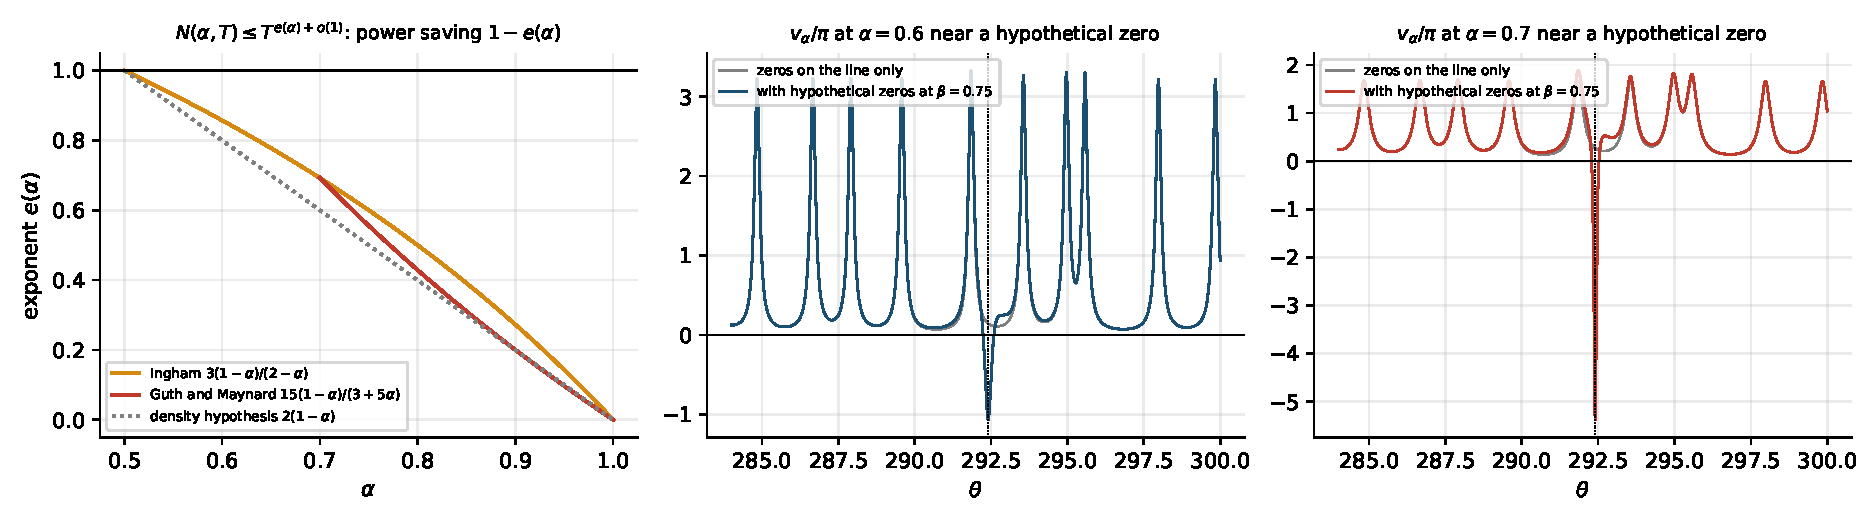
\includegraphics[width=\textwidth]{fig/ag_almost.pdf}
\caption{Left: the zero density exponents of Theorem~\ref{ag:thm:almost} and the region where they give a power saving; the exponent of Guth and Maynard is drawn on $[\frac7{10},1)$, where it holds by their estimate and, above $\frac45$, by Huxley's \cite{Huxley72}. Middle and right: the density $v_\alpha/\pi$ at $\alpha=0.6$ and $0.7$ near the hypothetical off line zero at height $292.4$ (dotted), with and without the hypothetical zeros, evaluated as in \texttt{almost.py} with step $0.005$. Drawn by \texttt{figs\_almost.py}.}
\label{ag:fig:almost}
\end{figure}

\subsection{Positivity margins and the circular unitary ensemble}\label{ag:sec:margins}

By Lemma~\ref{ag:lem:cancel}, a zero to the right of $\alpha$ at height $\gamma$ can make the density negative only if its distance to the line $\re s=\alpha$ is below $1/(\pi m)$, where $m$ is the local minimum of the rest of the density. The distribution of the local minima, the positivity margins, therefore determines how much room RH has at each height. The minima occur between consecutive ordinates. After unfolding the ordinates to unit mean spacing, $x_n=\vartheta(\gamma_n)/\pi+1$ with $\vartheta$ the Riemann Siegel theta function, as in Section~\ref{sec:ch15:spacings}, the density at the resolution of $\kappa$ mean spacings is
\[
\bar\rho_\kappa(x)=\sum_nP_\kappa(x-x_n)=\sum_n\frac{\kappa}{\pi(\kappa^2+(x-x_n)^2)},
\]
whose mean is one.

The script \texttt{sens.py} evaluates $\bar\rho_\kappa$ at the $1600$ midpoints between consecutive unfolded ordinates below height $2198$, leaving out $50$ mean spacings at each end, and the same statistic at about $3600$ midpoints between the eigenvalues of twelve Haar distributed unitary matrices of size $400$, unfolded and extended periodically. The circular unitary ensemble (CUE) of these matrices models the local statistics of the zeros. Table~\ref{ag:tab:margin} shows the result. The medians agree to $1\%$ at every resolution. In the lower tail the zeros have slightly larger margins than the CUE, a finite height effect in the expected direction, since the low zeros are more rigid than the limit of large matrices.

\begin{table}[htbp]
\centering\small
\begin{tabular}{ccccccc}
\toprule
$\kappa$ & zeta, 0.1\% & CUE, 0.1\% & zeta, 1\% & CUE, 1\% & zeta, median & CUE, median\\
\midrule
0.1 & 0.1075 & 0.0919 & 0.1177 & 0.1095 & 0.3349 & 0.3343\\
0.25 & 0.2617 & 0.2178 & 0.2849 & 0.2659 & 0.7116 & 0.7092\\
0.5 & 0.4803 & 0.4047 & 0.5150 & 0.4645 & 0.9739 & 0.9796\\
1 & 0.7477 & 0.6552 & 0.7730 & 0.7313 & 1.0264 & 1.0240\\
\bottomrule
\end{tabular}
\caption{Quantiles of the normalised Thorin density $\bar\rho_\kappa$ at the midpoints between consecutive unfolded ordinates, for the zeros below height $2198$ and for CUE eigenvalues. Computed by \texttt{sens.py}.}
\label{ag:tab:margin}
\end{table}

The next step is to repeat the comparison with Odlyzko's tables of zeros near the $10^{12}$th zero \cite{Odlyzko87} and near the $10^{21}$st and $10^{22}$nd zeros \cite{Odlyzko01,OdlyzkoTables}, where the finite height corrections are smaller, and to fit the lower tail of the margin distribution. The CUE lower tail is governed by large gaps, whose probability decays like a Gaussian in the gap length, so the smallest margin among the first $N$ midpoints should decrease only like a power of $\sqrt{\log N}$. Converted through the cancellation lemma, this predicts the width, as a function of the height, of the strip to the right of each basepoint in which an off line zero could hide without being cancelled. That is the quantitative input that question (1) of Section~\ref{ag:sec:exactly} needs.

\subsection{Moments of zeta, the Barnes function and zero density}\label{ag:sec:moments}

The strength of Theorem~\ref{ag:thm:almost} is set by the zero density exponents, which rest on mean value estimates on the critical line, Ingham's on the fourth moment of $\zeta$. Keating and Snaith \cite{KS00} modelled $\zeta(\frac12+it)$ by the characteristic polynomial $Z_N(\theta)=\det(I-Ae^{-i\theta})$ of a Haar distributed unitary matrix $A$ of size $N$, a matrix of the circular unitary ensemble of Section~\ref{ag:sec:margins}, with $N$ in the role of $\log(T/2\pi)$. By analogy with the exact formula
\[
\E|Z_N(\theta)|^{2k}=\prod_{j=1}^N\frac{\Gamma(j)\Gamma(j+2k)}{\Gamma(j+k)^2}\sim\frac{\mathsf G(1+k)^2}{\mathsf G(1+2k)}\,N^{k^2},\qquad N\to\infty,
\]
they conjectured that the moments of $\zeta$ grow in the same way, with $\log(T/2\pi)$ in place of $N$ and an arithmetic factor $a_k$ in front (Section~\ref{ag:sec:ks}). Here $\mathsf G$ is the Barnes $G$ function, $\mathsf G(1+z)=\Gamma(z)\mathsf G(z)$ with $\mathsf G(1)=1$, written in sans serif to keep $G$ for the clock of Section~\ref{ch:clock}. Nikeghbali and Yor \cite{NY09} gave the random matrix factor a probabilistic meaning in GGC language: the Mellin transform of $|Z_N|$ and the Barnes function are expressed through products and sums of independent gamma, beta and log gamma variables, and the reciprocal of $\mathsf G$ has a L\'evy Khintchine type representation. The source of these representations is the decomposition of Bourgade, Hughes, Nikeghbali and Yor \cite{BHNY08},
\[
Z_N\stackrel d=\prod_{j=1}^N\Big(1+e^{i\omega_j}\sqrt{B_{1,j-1}}\Big),
\]
with independent angles $\omega_j$ uniform on $[0,2\pi)$ and independent beta variables $B_{1,j-1}$ with parameters $1$ and $j-1$, where $B_{1,0}=1$.



\subsubsection{The Keating and Snaith moments}\label{ag:sec:ks}

Write $I_k(T)=\frac1T\int_0^T|\zeta(\frac12+it)|^{2k}dt$. The conjecture of Keating and Snaith \cite{KS00}, in the form of Conrey, Farmer, Keating, Rubinstein and Snaith \cite{CFKRS05}, is
\[
I_k(T)\sim a_k\,\frac{\mathsf G(1+k)^2}{\mathsf G(1+2k)}\Big(\log\frac T{2\pi}\Big)^{k^2},\qquad a_k=\prod_p\Big(1-\frac1p\Big)^{k^2}\sum_{m\ge0}\Big(\frac{\Gamma(m+k)}{m!\,\Gamma(k)}\Big)^2p^{-m},
\]
the product of an arithmetic factor from the primes and the random matrix factor. It is a theorem for $k=1$ and $k=2$ and open for $k\ge3$. For $k=1$ Hardy and Littlewood \cite{HL16} proved the leading term, and Ingham \cite{Ingham26} the mean square with its secondary term, $I_1(T)=\log\frac T{2\pi}+2\gamma_E-1+o(1)$; for $k=2$ Ingham \cite{Ingham26} proved the asymptotic with the leading coefficient $\frac1{2\pi^2}$. The local factor of $a_k$ is $(1-\frac1p)^{k^2}{}_2F_1(k,k;1;\frac1p)$. Since ${}_2F_1(1,1;1;x)=(1-x)^{-1}$ and ${}_2F_1(2,2;1;x)=(1+x)(1-x)^{-3}$, it equals $1$ for $k=1$ and $1-p^{-2}$ for $k=2$, so that $a_1=1$ and $a_2=\prod_p(1-p^{-2})=6/\pi^2$ exactly. The Euler product over the primes below $2\times10^5$ gives $a_3=0.0493218$ (\texttt{repro/ks\_ak.py}); since the local factor for $k=3$ is $1-9p^{-2}+O(p^{-3})$, the omitted primes lower it by a relative $9\sum_{p>2\times10^5}p^{-2}\approx4\times10^{-6}$, to about $0.0493217$. With $\mathsf G(3)^2/\mathsf G(5)=\frac1{12}$ and $\mathsf G(4)^2/\mathsf G(7)=\frac1{8640}$ the leading coefficients are $1$, $0.0506606=\frac1{2\pi^2}$, which is Ingham's constant, and $5.709\times10^{-6}$, the value $42a_3/9!$ of \cite{CFKRS05}.

Table~\ref{ag:tab:moments}, computed by \texttt{ks.py}, compares the moments with the leading terms. For $k=1$ the full asymptotic is already accurate at $T=1000$. For $k=2$ and $k=3$ the leading term is a small part of the moment at these heights, because the lower order terms of the polynomial in $\log T$ predicted in \cite{CFKRS05} dominate.

\begin{table}[htbp]
\centering\small
\begin{tabular}{ccccccc}
\toprule
$T$ & $I_1(T)$ & $\log\frac T{2\pi}+2\gamma_E-1$ & $I_2(T)$ & leading, $k=2$ & $I_3(T)$ & leading, $k=3$\\
\midrule
125 & 3.062 & 3.145 & 28.0 & 4.05 & 396 & 0.11\\
250 & 3.869 & 3.838 & 53.1 & 9.33 & 1136 & 0.71\\
500 & 4.550 & 4.531 & 84.8 & 18.6 & 2632 & 3.36\\
1000 & 5.211 & 5.224 & 127.2 & 33.5 & 5309 & 12.6\\
\bottomrule
\end{tabular}
\caption{Moments of $\zeta$ on the critical line against the asymptotic of Hardy, Littlewood and Ingham for $k=1$ and the leading Keating and Snaith terms for $k=2$ and $3$. Computed by \texttt{ks.py}.}
\label{ag:tab:moments}
\end{table}

\subsubsection{The moments as exponential moments of the Thorin density}

The densities $v_\sigma$ are the derivatives of $\log|\xi|$ across the basepoints: $\frac\partial{\partial\sigma}\log|\xi(\sigma+it)|=\re\frac{\xi'}{\xi}(\sigma+it)=v_\sigma(t)$ wherever $\xi(\sigma+it)\ne0$. Integrating from the critical line to the basepoint one, for every $t$ such that $\xi$ has no zero on the segment from $\frac12+it$ to $1+it$, which excludes only countably many $t$,
\begin{equation}\label{ag:eq:logxi}
\log|\xi(\tfrac12+it)|=\log|\xi(1+it)|-\int_{1/2}^1v_a(t)\,da .
\end{equation}
The moments concern $\zeta$, not $\xi$. With the gamma factor $h(s)=\frac12s(s-1)\pi^{-s/2}\Gamma(\frac s2)$, so that $\xi=h\zeta$, the identity becomes
\[
|\zeta(\tfrac12+it)|^{2k}=|\zeta(1+it)|^{2k}\,\Big|\frac{h(1+it)}{h(\frac12+it)}\Big|^{2k}\exp\Big\{-2k\int_{1/2}^1v_a(t)\,da\Big\},
\]
and Stirling's formula gives $|h(1+it)/h(\frac12+it)|\sim(t/2\pi)^{1/4}$ as $t\to\infty$. So the Keating and Snaith moments are exponential moments, over $t$ uniform on $[0,T]$, of the density $v_a(t)$ integrated across the basepoints from $\frac12$ to $1$, with the weight $|\zeta(1+it)|^{2k}|h(1+it)/h(\frac12+it)|^{2k}$, which involves no zero of $\zeta$. In the same terms, RH, which is the positivity of $v_a$ for every $a>\frac12$ (Lagarias's criterion, Remark~\ref{rem:ch2:oneline}), is the statement that $|\xi(\sigma+it)|$ increases with $\sigma\ge\frac12$ for every $t$, a reformulation due to Sondow and Dumitrescu \cite{SD10}.

In the language of \eqref{ag:eq:logxi} the conjecture of Keating and Snaith is a large deviation statement for the integrated Thorin density. Selberg's central limit theorem \cite{Selberg46} says that for $t$ uniform on $[T,2T]$ the variable $\log|\zeta(\frac12+it)|$ is approximately Gaussian with variance $\frac12\log\log T$. Gaussian exponential moments would give $(\log T)^{k^2}$, and the constant $a_k\mathsf G(1+k)^2/\mathsf G(1+2k)$ is the correction to them. On $[500,1000]$ the sample variance of $\log|\zeta(\frac12+it)|$ is $1.53$, against $\frac12\log\log750=0.95$. The difference is a constant term, not slow convergence: the random matrix model predicts the variance $\frac12\log\log\frac t{2\pi}+c+o(1)$ with $c=\frac12\big(\gamma_E+1-\sum_p\sum_{m\ge2}(\frac1m-\frac1{m^2})p^{-m}\big)=0.70$ \cite{KS00}, a conjecture, and this gives $1.48$ on $[500,1000]$, close to the sample value.

\subsubsection{What the moments give}

Ingham's exponent $3(1-\sigma)/(2-\sigma)$, which gives Theorem~\ref{ag:thm:almost} its saving $(2\alpha-1)/(2-\alpha)$ for $\frac12<\alpha<\frac7{10}$, rests on the fourth moment, $k=2$, proved by Ingham \cite{Ingham26}. Bounds for all moments, that is the Lindel\"of hypothesis in the form $\int_0^T|\zeta(\frac12+it)|^{2k}dt\ll T^{1+\varepsilon}$ for every $k$, imply the density hypothesis $N(\sigma,T)\ll T^{2(1-\sigma)+\varepsilon}$, which would give the saving $2\alpha-1$, larger than that of Theorem~\ref{ag:thm:almost} for $\frac12<\alpha<\frac9{10}$. The Keating and Snaith asymptotics would give this and much more.

The GGC structure of Nikeghbali and Yor belongs to the random matrix model, not to $\zeta$: it explains the conjecture without proving it, and only the second and fourth moments of $\zeta$ are known asymptotically. And moments, even the Lindel\"of hypothesis, bound the number of zeros off the line but do not exclude them.

\subsection{From almost to exactly}\label{ag:sec:exactly}

Theorem~\ref{ag:thm:almost} cannot be upgraded to exact positivity by improving the exponents, or by the moment bounds of Section~\ref{ag:sec:moments}. Even the density hypothesis, or the Lindel\"of hypothesis which implies it, leaves room for a sparse set of zeros off the line, and a single off line zero $\beta+i\gamma$ stops $T_\alpha$ from being a GGC for every $\alpha$ in $[\frac12,\beta)$ (Theorem~\ref{thm:poisson}) and makes $v_\alpha$ negative near $\gamma$ for every $\alpha$ close enough to $\beta$ (Section~\ref{ag:sec:cancel}). The step from ``almost'' to ``exactly'' is a step from counting zeros to excluding them.

Four facts about the programme say that this step needs input from outside it. The smoothing runs the wrong way: when no zero lies to the right of $\alpha$ the density at a basepoint $\alpha'>\alpha$ is the Poisson smoothing of the density at $\alpha$ by the kernel of width $\alpha'-\alpha$, and positivity propagates to the right; RH asks to propagate it to the left, which is deconvolution, and deconvolution does not preserve positivity. Arithmetic domination requires a zero free region: below the basepoint one the compensated L\'evy form, which the sine squared lemma converts into the density, holds if $\psi(x)-x=O(x^{\alpha'})$ for some $\alpha'<\alpha$, and only if $\psi(x)-x=O(x^{\alpha+\delta})$ for every $\delta>0$, where $\psi$ is Chebyshev's function (Proposition~\ref{bp:prop:below}). Either condition is a zero free half plane, none was known for any $\alpha<1$ before the half plane $\re s>\frac78$ announced in October 2026, which came from outside the programme (Section~\ref{sec:ch25:open}), and removing the pole does not help: for $L(s,\chi_{12})$ the prime sums need no compensation, and the boundary is the same (Section~\ref{bp:eta:sec:below}). There is no margin: along the de Bruijn Newman flow the reciprocal is a GGC for $t\ge0.2$ \cite{PT21} (Theorem~\ref{rz:thm:dbn} and Section~\ref{ch:dbn}), RH is the statement at $t=0$, and $\Lambda\ge0$ \cite{RodgersTao}, so a proof must establish a closed condition at the boundary itself. And stronger positivity conditions can be false: Conrey and Li showed that a positivity condition in de Branges' approach to RH fails \cite{CL00}, so any positivity statement stronger than RH should be tested numerically before it is pursued (Section~\ref{st:sec:wp5}).

In the Stieltjes form (iv) of Theorem~\ref{bh:thm:main} the difference between counting zeros and excluding them is explicit. Split $G'/G=S_{\rm on}+R_{\rm off}$, where $S_{\rm on}(u)=\sum(u+\gamma^2)^{-1}$ runs over the zeros $\frac12+i\gamma$ on the line with $\gamma>0$ and is a Stieltjes function with measure $U_{\rm line}$, and $R_{\rm off}(u)=\sum(u-(\rho-\frac12)^2)^{-1}$ runs over the zeros $\rho=\beta+i\gamma$ off the line with $\gamma>0$. By Theorem~\ref{bs:thm:local}, all the poles of $R_{\rm off}$ lie in a parabolic sliver $\mathcal E_{T_0}$ beside the negative axis, which begins at $-T_0^2+T_0+\frac14$, and in the upper half plane outside it $\im R_{\rm off}\le0$ and $\im(G'/G)<0$. The size of $R_{\rm off}$ away from the sliver needs no count of zeros: if $|u|\le T_0^2/2$, a disc that misses $\mathcal E_{T_0}$, then every term has $|u-(\rho-\frac12)^2|\ge|\rho-\frac12|^2-|u|>\gamma^2/2$, since $\gamma>T_0$, so $|R_{\rm off}(u)|\le2\Sigma_0<3\times10^{-12}$ by Theorem~\ref{ag:thm:explicit}.

The number of terms of $R_{\rm off}$, on the other hand, is not known to be small. Zero density estimates bound the number of those with $|\beta-\frac12|\ge\sigma-\frac12$ and $\gamma\le T$ by $T^{e(\sigma)+o(1)}$ with $e(\sigma)<1$, for each fixed $\sigma>\frac12$ (Theorem~\ref{ag:thm:almost}), which is $o(T)$; but zeros off the line may approach the line as $\gamma$ grows, and for all of them together only a proportion is known. At most $(1-\kappa+o(1))N(T)$ of the zeros up to height $T$ lie off the line, with $\kappa>\frac5{12}$ in the last published record \cite{PRZZ20} and $\kappa>0.6725$, counting only simple zeros on the line, in two preprints of 2026 \cite{AF26,Lam26}; that is not $o(T)$, nor even $o(N(T))$. No count, however strong, touches the Thorin condition, which requires $R_{\rm off}\equiv0$, because a single pair puts a pole of $G'/G$ off the cut. Section~\ref{pk:sec:filter} gives a test for arguments that claim to exclude such poles: since the de Bruijn Newman flow has nonreal zeros at every $t<0$ \cite{RodgersTao}, no property that the kernel $e^{tv^2/4}\Phi(v)$ keeps for some $t<0$ can exclude them, so a proof must use one that fails for every $t<0$, and the Euler product and the explicit formula are the natural candidates.

The forms that the new input could take are those of Section~\ref{ch:path}. The first new theorem any of them would give is the GGC property of $T_\alpha$ at a single basepoint $\alpha<\frac78$, that is $v_\alpha^-\equiv0$, a zero free half plane beyond the one announced in 2026 (Section~\ref{sec:ch25:open}); positivity of $v_\alpha$ on the single line $\re s=\alpha$ is not known to suffice (Remark~\ref{rem:ch2:oneline}).

Sections~\ref{ag:sec:factor} and \ref{ag:sec:cancel} make the remaining problem concrete. The growth of the defect is not part of it. For $u\ge1$ every factor of $D_\alpha$ is at most one, and a factor with $\gamma\le\sqrt u$ is at least $\gamma^2/(u+\gamma^2)\ge\gamma^2/(2u)\ge1/u$, since $\gamma\ge\gamma_1>\sqrt2$. Bounding the factors with $\gamma>\sqrt u$ as in the proof of Theorem~\ref{ag:thm:explicit} therefore gives, for $u\ge1$,
\begin{align*}
|\log D_\alpha(u)|&\le N(\alpha,\sqrt u)\log u+2(u+\sqrt u)\sum_{\beta>\alpha,\ \gamma>\sqrt u}\gamma^{-2}\\
&\le u^{e(\alpha)/2+o(1)},\qquad u\to\infty,
\end{align*}
by the exponents of Theorem~\ref{ag:thm:almost}. So bounds on the growth of the defect follow from zero density estimates alone, and what remains open is whether it is identically one. Four questions would each be a genuine step.
\begin{enumerate}
\item Cancellation on average: show that for fixed $\alpha>\frac12$ the background density $v_\alpha/\pi$ is bounded below by $c\log\gamma$ outside a set of heights of density zero. With Lemma~\ref{ag:lem:cancel} this would confine any failure of positivity to zeros in the strips $\alpha<\beta<\alpha+O(1/\log\gamma)$. Remark~\ref{rem:dbeta:average} proves the lower bound for $v_\alpha/\pi$ itself, but its exceptional set contains a neighbourhood of the ordinate of every zero to the right of $\alpha$, which is where Lemma~\ref{ag:lem:cancel} would need it.
\item Thin strip density: bound the number of zeros with $\alpha<\beta<\alpha+2/\log\gamma$ and $\gamma\le T$ by $o(T^{1-\delta})$ for some $\delta>0$, uniformly in $\alpha$. Combined with (1) this would give a pointwise almost positivity theorem.
\item Explicit defect: bound $\log D_\alpha(u)$ explicitly, as described at the end of Section~\ref{ag:sec:factor}.
\item Positivity at one basepoint: prove $D_\alpha\equiv1$, that is $v_\alpha^-\equiv0$, for a single $\alpha<\frac78$, which is a zero free half plane beyond the one announced in 2026 (Section~\ref{sec:ch25:open}).
\end{enumerate}
What the Thorin framework contributes is a precise target, the GGC property of one explicit clock $T_\alpha$ at one basepoint below $\frac78$, together with computational tools that test candidate arguments against it: certified densities on windows, positivity margins calibrated against random matrix theory, and the explicit defect. Chapter~\ref{chap:conclusions} takes stock of the whole path, beginning with Section~\ref{ch:path}.
